\documentclass[border=4pt]{standalone}
\usepackage[T1]{fontenc}
\usepackage{amsmath}
\usepackage{tikz}
\usetikzlibrary{arrows.meta, shapes.geometric, fit, backgrounds, calc}

\begin{document}
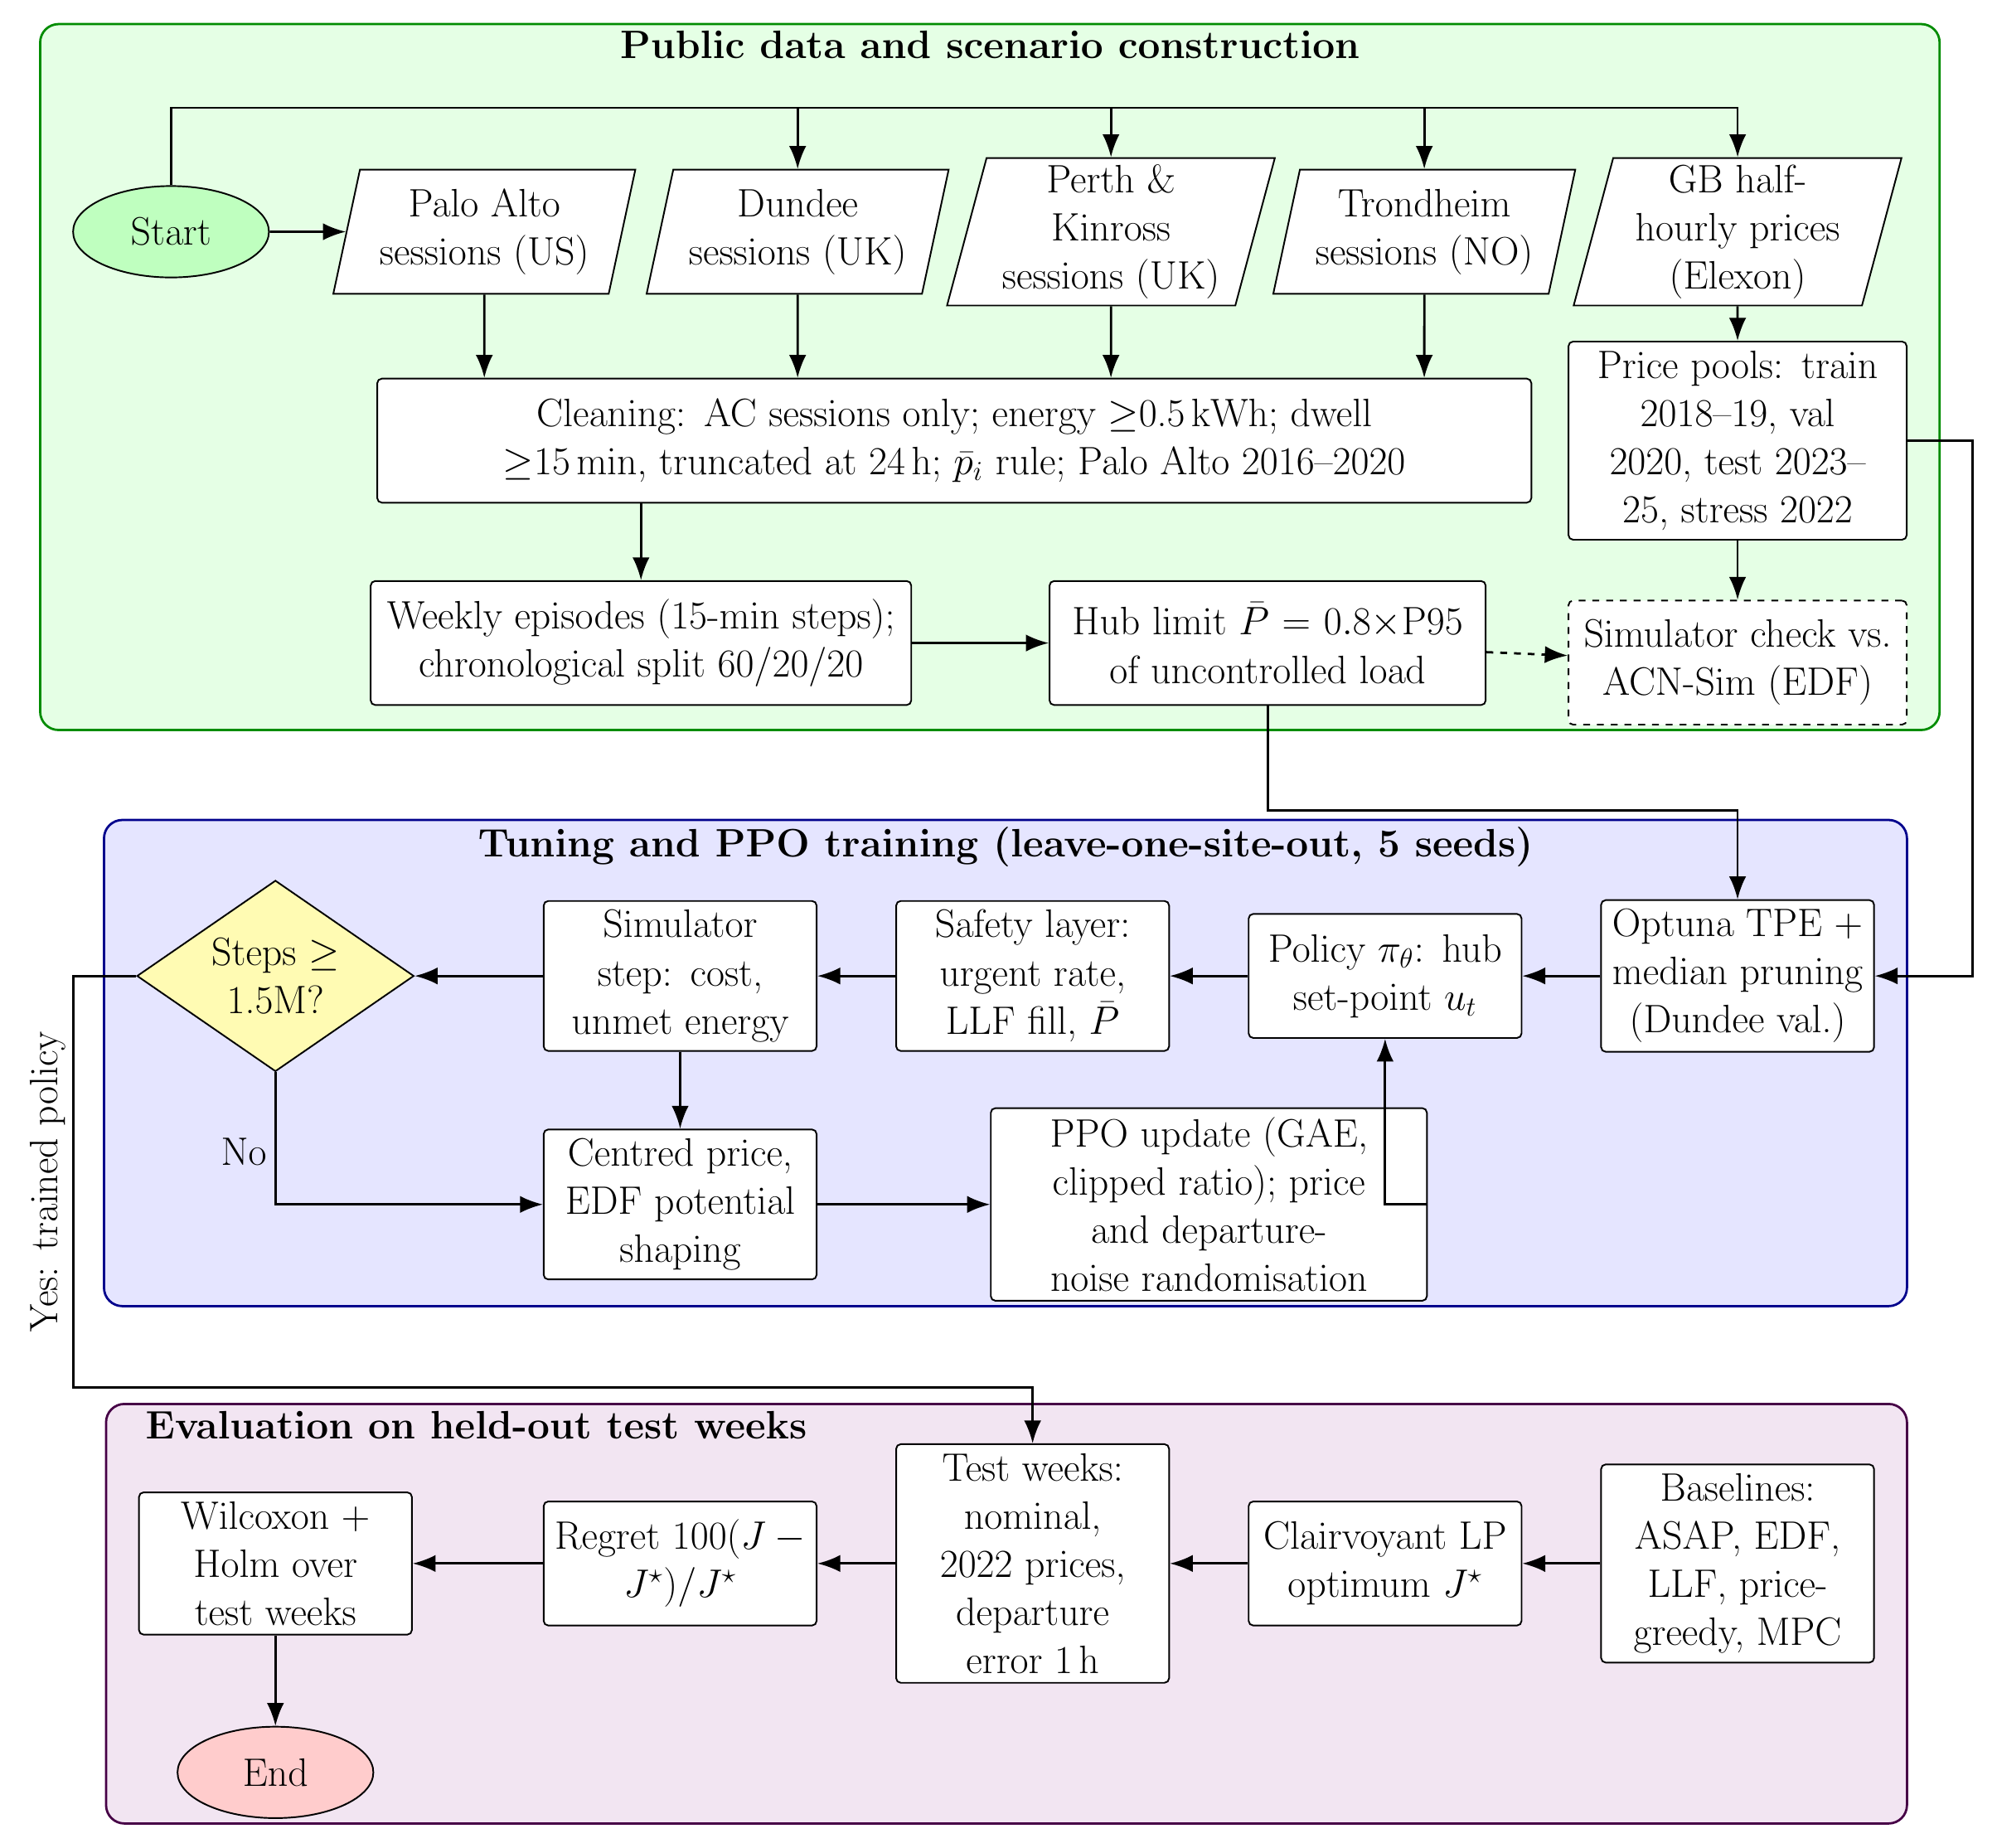
\begin{tikzpicture}[
    x=1cm, y=1cm,
    font=\fontsize{18}{21}\selectfont,
    every node/.style={align=center},
    box/.style={rectangle, rounded corners=2pt, draw=black, line width=0.7pt, text width=3.9cm, minimum height=1.9cm, inner sep=4pt, fill=white},
    data/.style={trapezium, trapezium left angle=75, trapezium right angle=105, trapezium stretches body, draw=black,
                 line width=0.7pt, text width=3.6cm, minimum height=1.9cm, inner sep=3pt, fill=white},
    dec/.style={diamond, aspect=1.45, draw=black, line width=0.7pt, text width=2.4cm, inner sep=1pt, fill=yellow!30},
    term/.style={ellipse, draw=black, line width=0.7pt, minimum width=3.0cm, minimum height=1.4cm, fill=green!25},
    stop/.style={ellipse, draw=black, line width=0.7pt, minimum width=3.0cm, minimum height=1.4cm, fill=red!20},
    arrow/.style={-{Latex[length=3.5mm]}, line width=1pt},
    darrow/.style={-{Latex[length=3.5mm]}, line width=1pt, dashed},
    region/.style={rounded corners=8pt, draw=#1!55!black, line width=1pt, fill=#1!10},
    rtitle/.style={font=\fontsize{18}{21}\selectfont\bfseries, anchor=north}
]

% ------------------------------------------------------------ data block (top)
\node[term] (start) at (1.8, 0.0) {Start};
\node[data] (pa)  at (6.6, 0.0)  {Palo Alto sessions (US)};
\node[data] (du)  at (11.4, 0.0) {Dundee sessions (UK)};
\node[data] (pe)  at (16.2, 0.0) {Perth \& Kinross sessions (UK)};
\node[data] (tr)  at (21.0, 0.0) {Trondheim sessions (NO)};
\node[data] (pr)  at (25.8, 0.0) {GB half-hourly prices (Elexon)};
\node[box, text width=17.4cm] (clean) at (13.8, -3.2) {Cleaning: AC sessions only; energy $\geq$0.5\,kWh; dwell $\geq$15\,min, truncated at 24\,h; $\bar p_i$ rule; Palo Alto 2016--2020};
\node[box, text width=4.9cm] (pools) at (25.8, -3.2) {Price pools: train 2018--19, val 2020, test 2023--25, stress 2022};
\node[box, text width=8.0cm] (weeks) at (9.0, -6.3) {Weekly episodes (15-min steps); chronological split 60/20/20};
\node[box, text width=6.4cm] (cap) at (18.6, -6.3) {Hub limit $\bar P = 0.8\times$P95 of uncontrolled load};
\node[box, dashed, text width=4.9cm] (val) at (25.8, -6.6) {Simulator check vs.\ ACN-Sim (EDF)};

% ------------------------------------------------------------ tuning and training block (middle)
\node[box] (hpo)  at (25.8, -11.4) {Optuna TPE + median pruning (Dundee val.)};
\node[box] (act)  at (20.4, -11.4) {Policy $\pi_\theta$: hub set-point $u_t$};
\node[box] (safe) at (15.0, -11.4) {Safety layer: urgent rate, LLF fill, $\bar P$};
\node[box] (sim)  at (9.6, -11.4)  {Simulator step: cost, unmet energy};
\node[box] (rew)  at (9.6, -14.9)  {Centred price, EDF potential shaping};
\node[dec] (done) at (3.4, -11.4)  {Steps $\geq$ 1.5M?};
\node[box, text width=6.4cm] (ppo) at (17.7, -14.9) {PPO update (GAE, clipped ratio); price and departure-noise randomisation};

% ------------------------------------------------------------ evaluation block (bottom)
\node[box] (base) at (25.8, -20.4) {Baselines: ASAP, EDF, LLF, price-greedy, MPC};
\node[box] (opt)  at (20.4, -20.4) {Clairvoyant LP optimum $J^\star$};
\node[box] (cond) at (15.0, -20.4) {Test weeks: nominal, 2022 prices, departure error 1\,h};
\node[box] (reg)  at (9.6, -20.4)  {Regret $100(J-J^\star)/J^\star$};
\node[box] (stat) at (3.4, -20.4)  {Wilcoxon + Holm over test weeks};
\node[stop] (end) at (3.4, -23.6)  {End};

% ------------------------------------------------------------ backgrounds
\begin{scope}[on background layer]
  \node[region=green, fit=(start)(pa)(pr)(clean)(weeks)(val), inner xsep=14pt, inner ysep=30pt, yshift=28pt] (bgA) {};
  \node[region=blue, fit=(done)(hpo)(rew)(ppo), inner xsep=14pt, inner ysep=14pt, yshift=12pt] (bgB) {};
  \node[region=violet, fit=(stat)(base)(end), inner xsep=14pt, inner ysep=14pt, yshift=12pt] (bgC) {};
\end{scope}
\node[rtitle] at (bgA.north) {Public data and scenario construction};
\node[rtitle] at (bgB.north) {Tuning and PPO training (leave-one-site-out, 5 seeds)};
\node[rtitle, anchor=north west] at ($(bgC.north west)+(0.5,0)$) {Evaluation on held-out test weeks};

% ------------------------------------------------------------ arrows
\draw[arrow] (start) -- (pa);
\draw[arrow] (start.north) |- (4.4, 1.9) -| (du.north);
\draw[arrow] (start.north) |- (4.4, 1.9) -| (pe.north);
\draw[arrow] (start.north) |- (4.4, 1.9) -| (tr.north);
\draw[arrow] (start.north) |- (4.4, 1.9) -| (pr.north);
\draw[arrow] (pa) -- (pa |- clean.north);
\draw[arrow] (du) -- (du |- clean.north);
\draw[arrow] (pe) -- (pe |- clean.north);
\draw[arrow] (tr) -- (tr |- clean.north);
\draw[arrow] (pr) -- (pools);
\draw[arrow] (clean.south -| weeks.north) -- (weeks.north);
\draw[arrow] (weeks) -- (cap);
\draw[arrow] (pools) -- (val);
\draw[darrow] (cap) -- (val);
\draw[arrow] (pools.east) -- ++(1.0,0) |- (hpo.east);
\draw[arrow] (cap.south) -- ++(0,-1.6) -| (hpo.north);

\draw[arrow] (hpo) -- (act);
\draw[arrow] (act) -- (safe);
\draw[arrow] (safe) -- (sim);
\draw[arrow] (sim) -- (done);
\draw[arrow] (sim) -- (rew);
\draw[arrow] (rew) -- (ppo);
\draw[arrow] (ppo.east) -| (act.south);
\draw[arrow] (done.south) |- node[left, pos=0.3] {No} (rew.west);
\draw[arrow] (done.west) -- (0.3, -11.4) |- node[pos=0.25, rotate=90, anchor=south, inner sep=3pt] {Yes: trained policy} (6.3, -17.7) -| (cond.north);

\draw[arrow] (base) -- (opt);
\draw[arrow] (opt) -- (cond);
\draw[arrow] (cond) -- (reg);
\draw[arrow] (reg) -- (stat);
\draw[arrow] (stat) -- (end);
\end{tikzpicture}
\end{document}
